\documentclass[tikz,border=2mm]{standalone}
\usepackage{amsmath,amssymb}
\usetikzlibrary{arrows.meta,positioning}
\newcommand{\tikzsetnextfilename}[1]{}

\tikzset{
  svrpp cell/.style={draw=black, line width=0.7pt, minimum width=2.1cm,
    minimum height=1.25cm, inner sep=2pt},
  equality mark/.style={<->,>=Stealth,line width=0.75pt},
  statistic/.style={font=\small,align=left}
}

\newcommand{\svrppCell}[3]{%
  \node[svrpp cell] at (#1,#2) {$#3$};%
}

\begin{document}

\tikzsetnextfilename{hybrid-grothendieck-example}
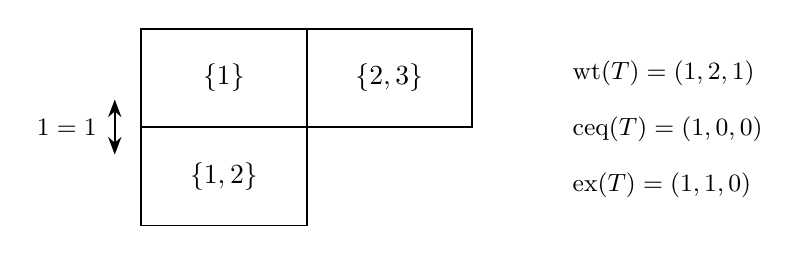
\begin{tikzpicture}[x=2.1cm,y=1.25cm]
  \svrppCell{0}{1}{\{1\}}
  \svrppCell{1}{1}{\{2,3\}}
  \svrppCell{0}{0}{\{1,2\}}

  \draw[equality mark] (-0.66,0.22) -- (-0.66,0.78)
    node[midway,left=1mm,font=\small] {$1=1$};

  \node[statistic,anchor=west] at (2.05,1.05)
    {$\operatorname{wt}(T)=(1,2,1)$};
  \node[statistic,anchor=west] at (2.05,0.48)
    {$\operatorname{ceq}(T)=(1,0,0)$};
  \node[statistic,anchor=west] at (2.05,-0.09)
    {$\operatorname{ex}(T)=(1,1,0)$};
\end{tikzpicture}

\end{document}
